\section{Frontend Implementation}
Frontend was written in JavaScript language using React library.

\subsection{Communication with backend}
Submit of the forms action was putting saveLessonItem(data parsed form fields in a form) and forward them to database using POST and PUT requests.
\begin{lstlisting}[breaklines=true, numbers=left, stepnumber=1]
const { data } = lessonItem === undefined ? (
    await fetchContext.authAxios.post(
      `/v1/lessons`,
      saveLessonItem
    )
  ) : (
      await fetchContext.authAxios.put(
        `/v1/lessons/` + saveLessonItem._id,
        saveLessonItem
      )
    );
\end{lstlisting}

Receiving data from backend was realized as getting data from database and setting variables with received data.  
\begin{lstlisting}[breaklines=true, numbers=left, stepnumber=1]
const { data } = await fetchContext.authAxios.get(
    '/v1/users/lessons'
  );
setLessonItems(data);
\end{lstlisting}

\subsection{User interface description}
Basic user operations as \textit{Login} and \textit{Sign Up} was shown at the figures \ref{fig:Login} and \ref{fig:SignUp}.
\begin{figure}[H]
    \centering
    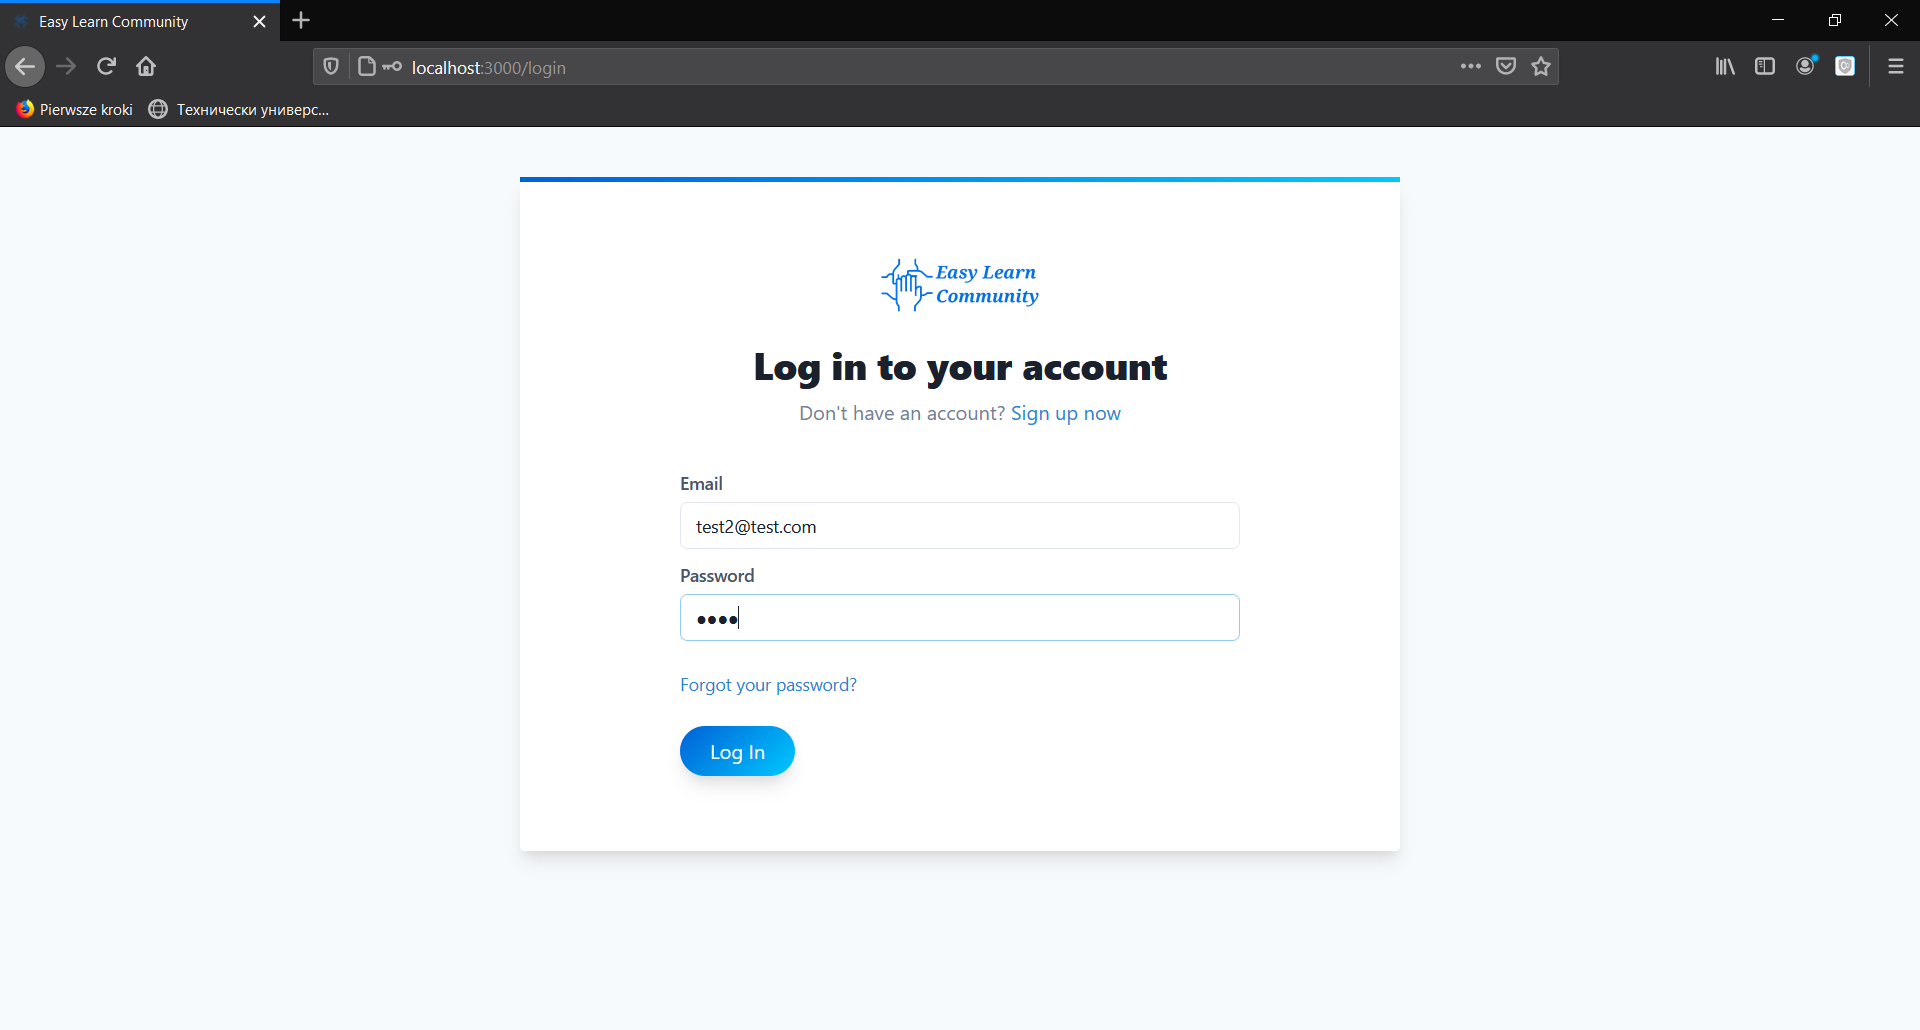
\includegraphics[width=\textwidth]{Include/Resources/Frontend/Login.png}
    \caption{Login view} 
    \label{fig:Login}
\end{figure}

\begin{figure}[H]
    \centering
    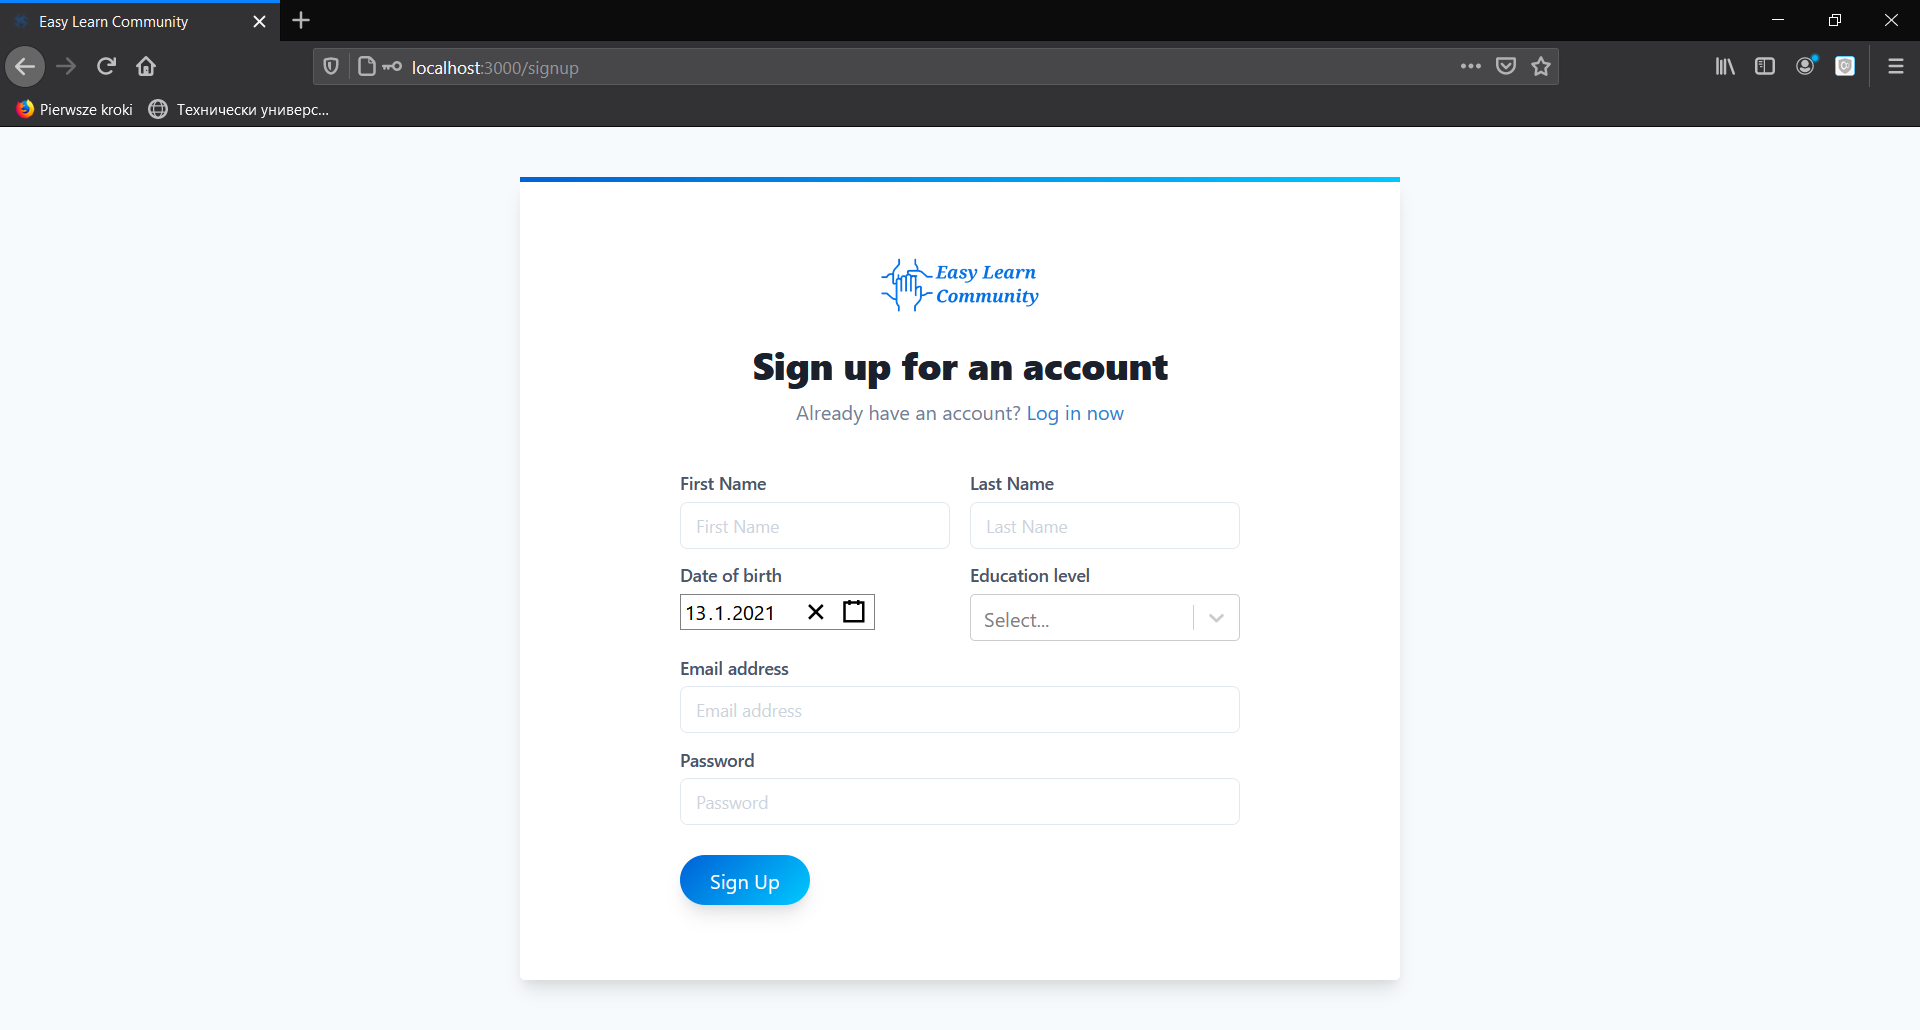
\includegraphics[width=\textwidth]{Include/Resources/Frontend/SignUp.png}
    \caption{Sign up view} 
    \label{fig:SignUp}
\end{figure}

Newly created user is set as student from default.

Student and Teacher can find a lesson(figure nr \ref{fig:FindLesson}), so they can improve their skills.

\begin{figure}[H]
    \centering
    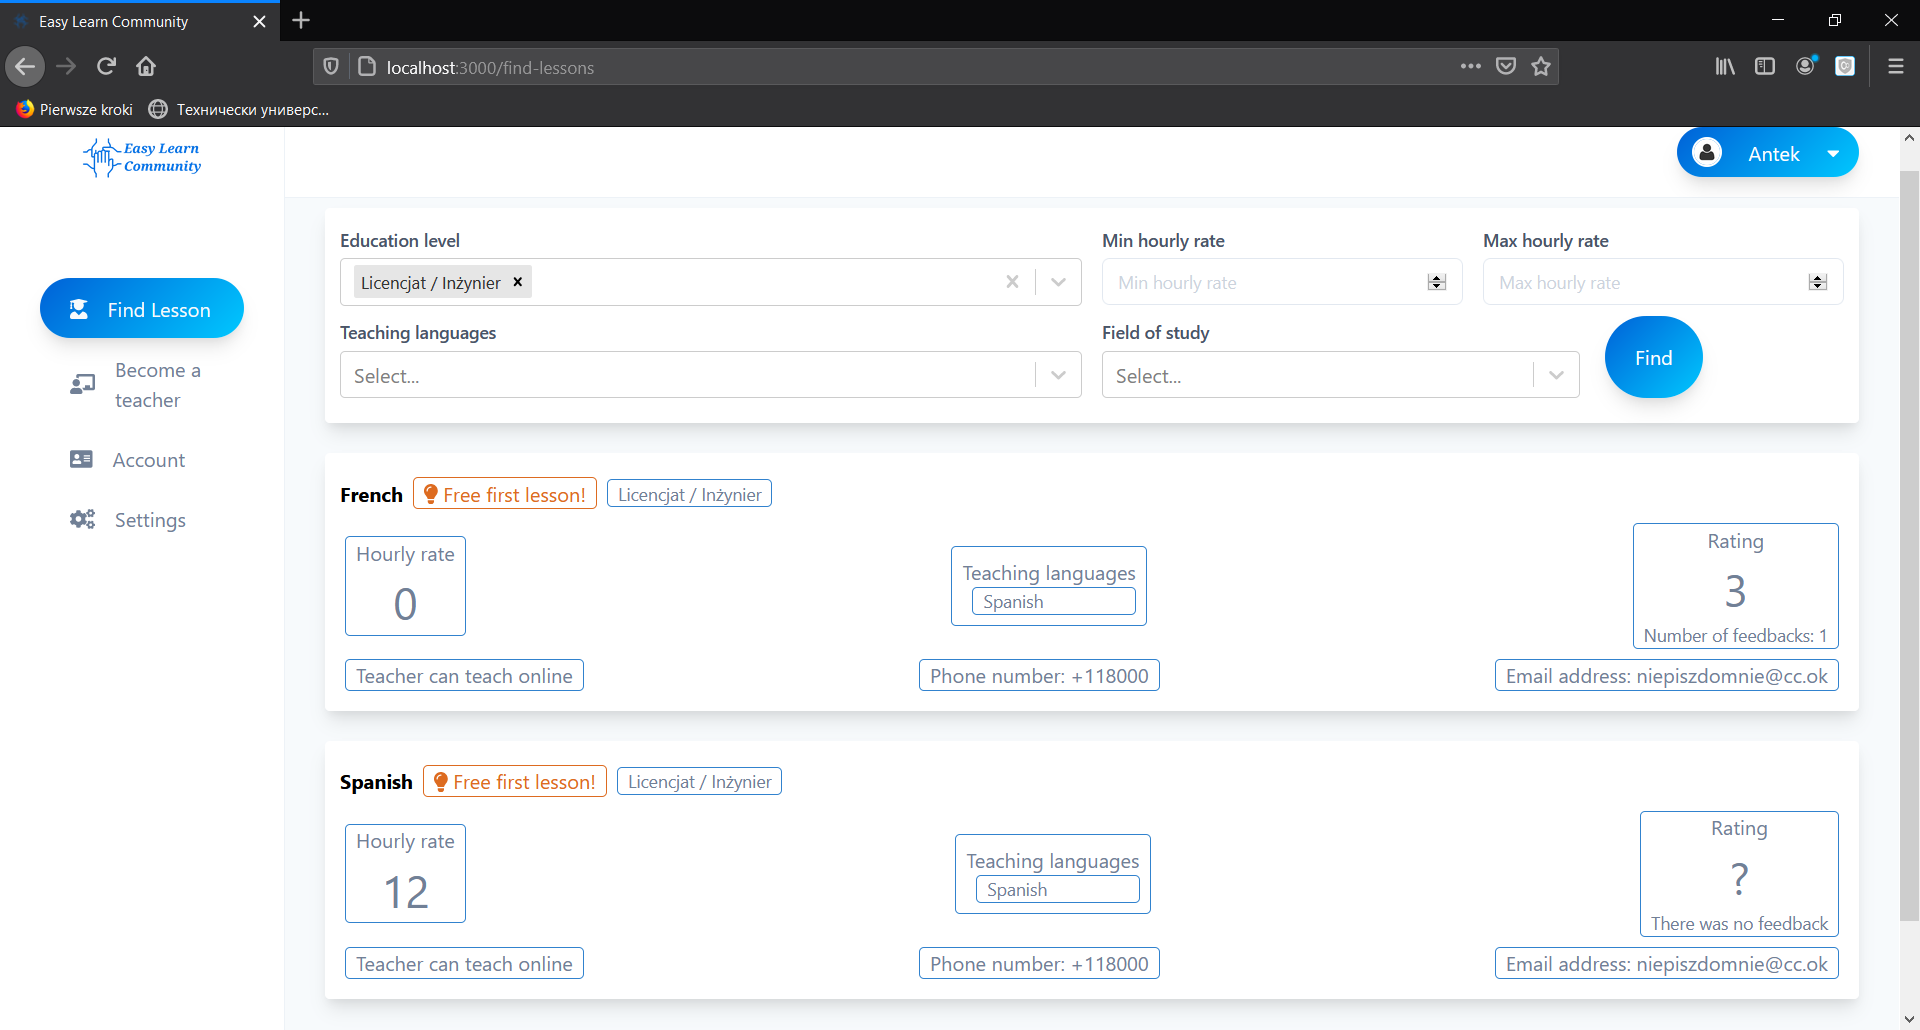
\includegraphics[width=\textwidth]{Include/Resources/Frontend/FindLesson.png}
    \caption{Find lesson view} 
    \label{fig:FindLesson}
\end{figure}

Student can become a teacher by selecting \textit{Become a teacher} tab, filling contact data(figure nr \ref{fig:BecomeATeacher1}) and adding new lesson item(figure nr \ref{fig:BecomeATeacher2}).
\begin{figure}[H]
    \centering
    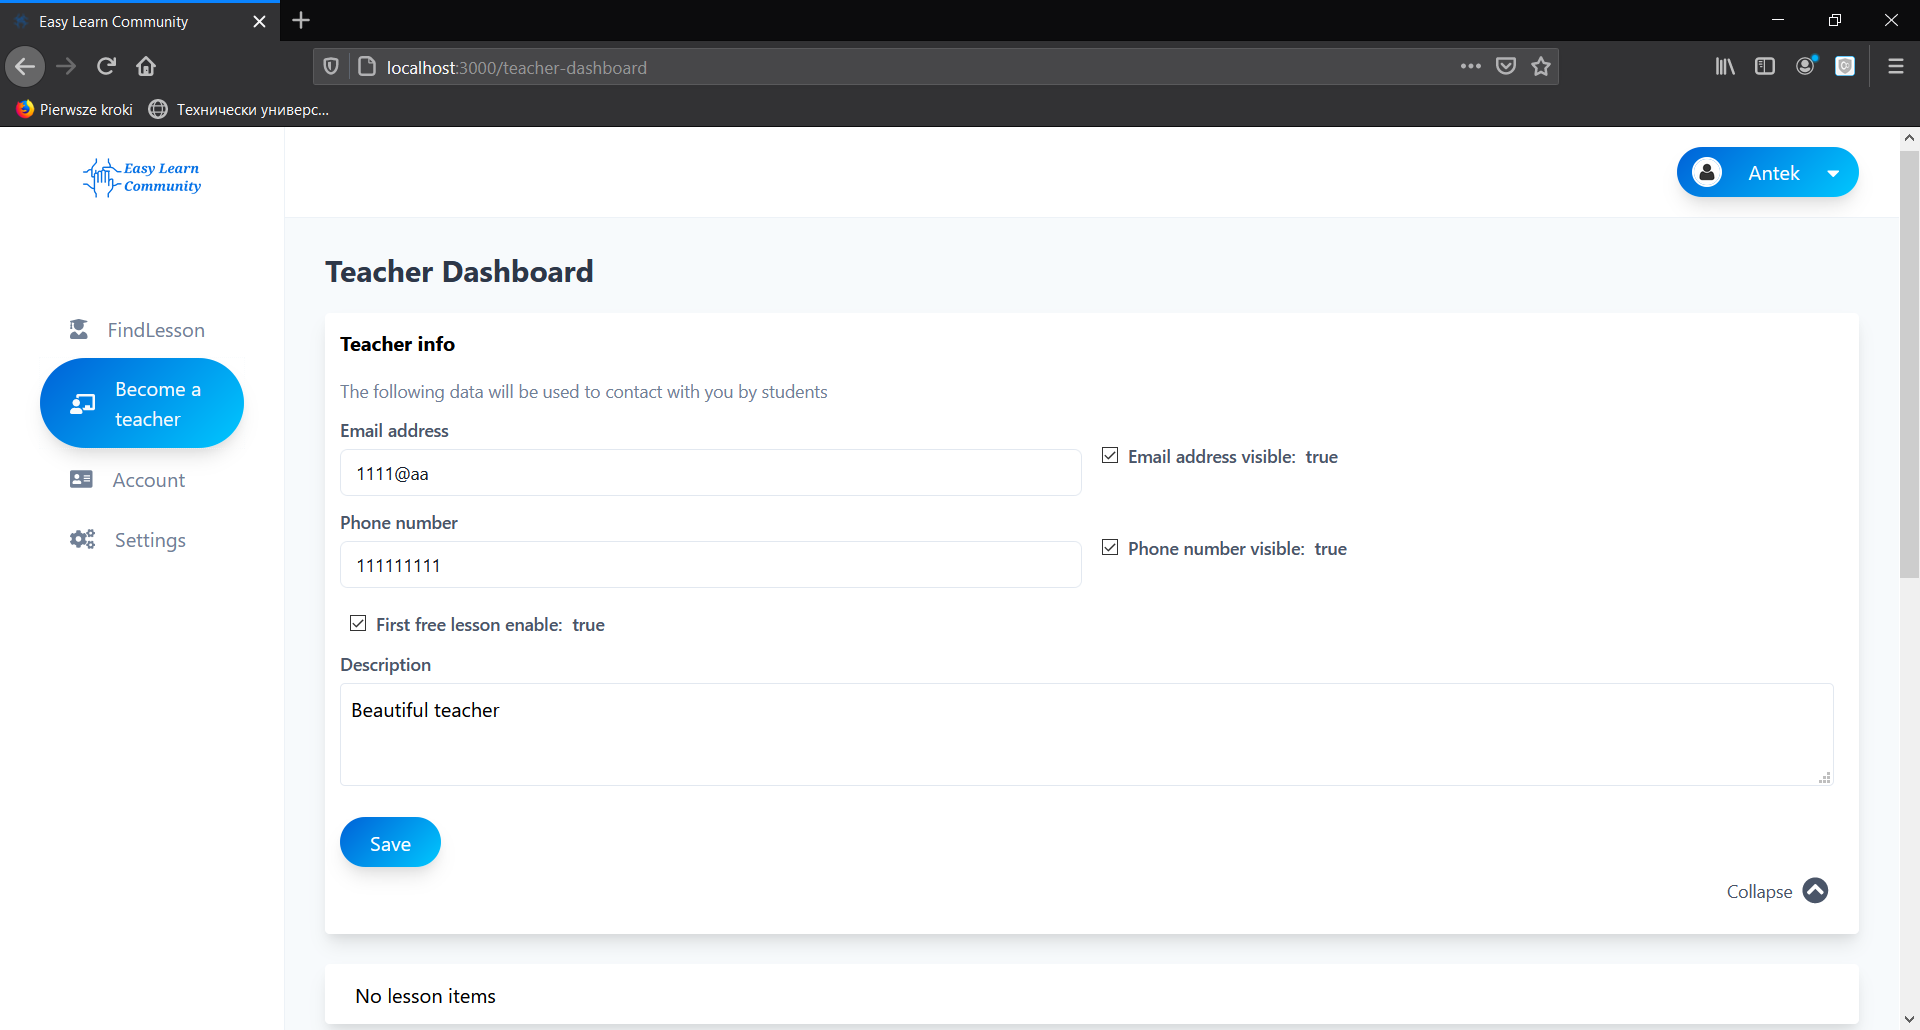
\includegraphics[width=\textwidth]{Include/Resources/Frontend/BecomeATeacher1.png}
    \caption{Become a teacher - fill contact data} 
    \label{fig:BecomeATeacher1}
\end{figure}

\begin{figure}[H]
    \centering
    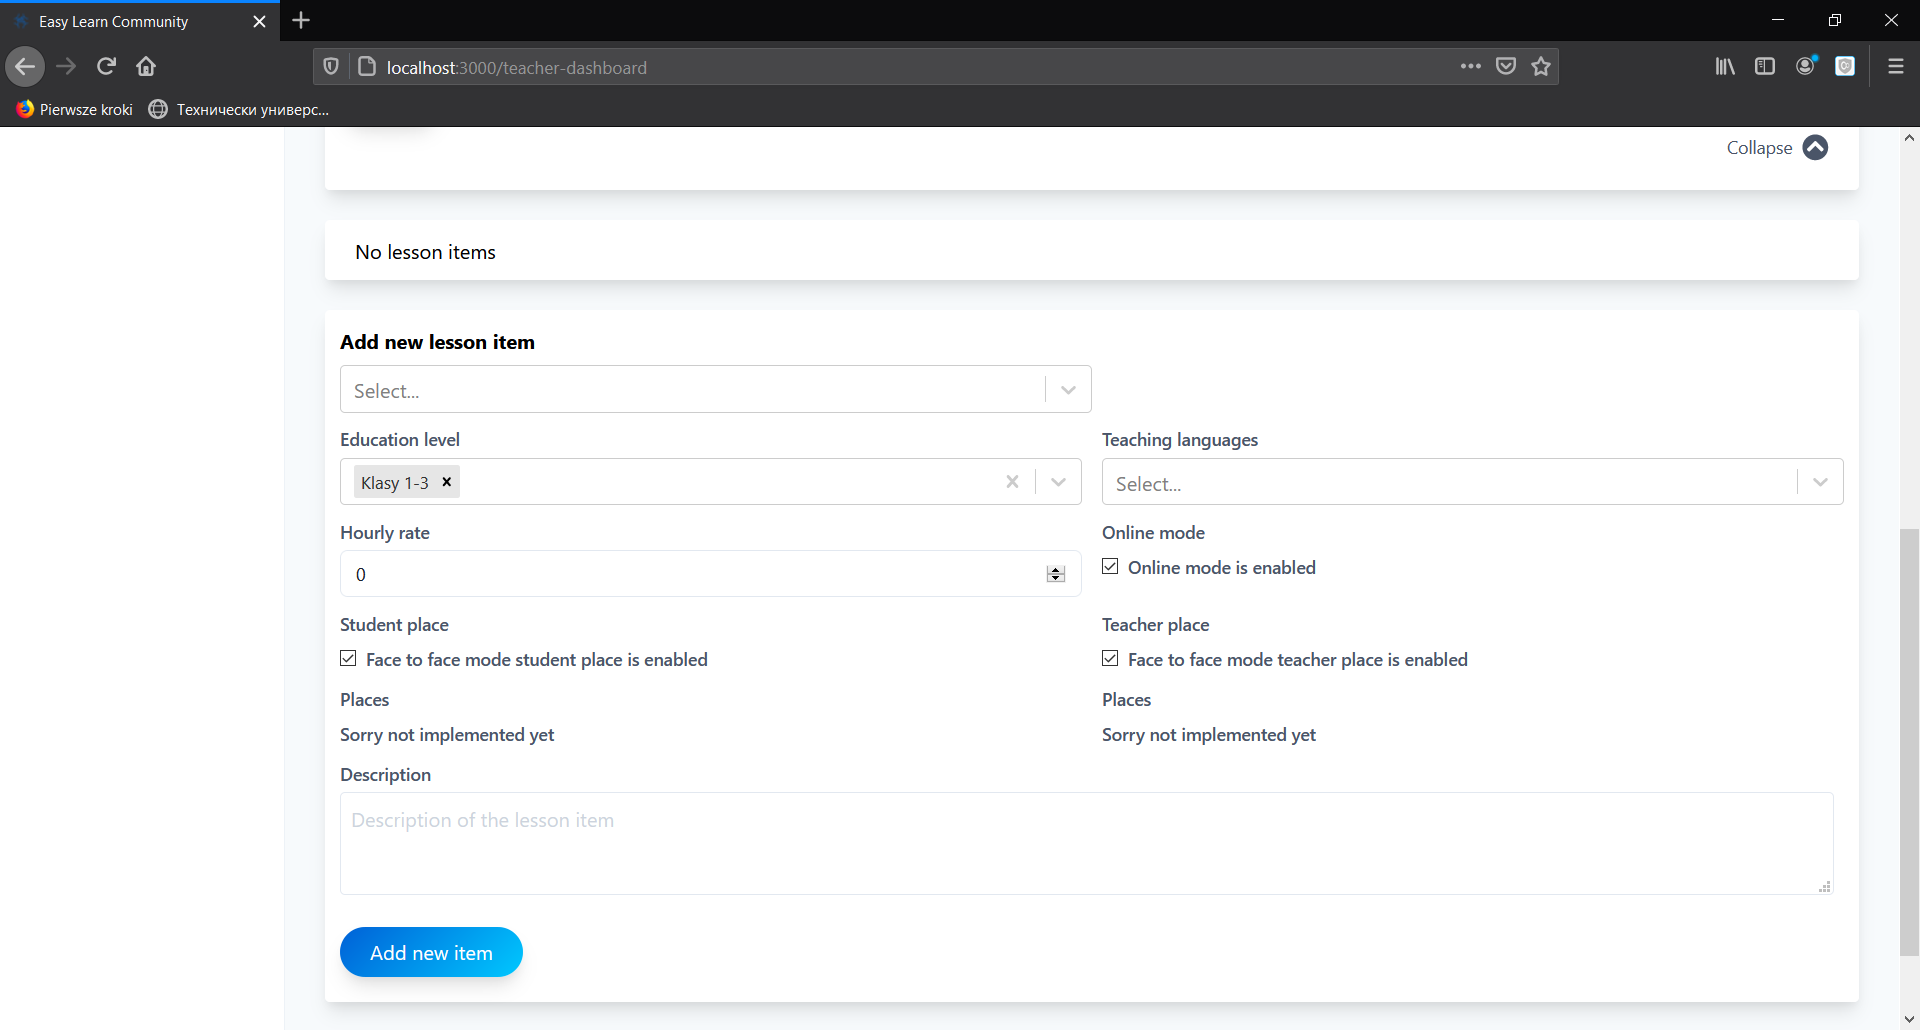
\includegraphics[width=\textwidth]{Include/Resources/Frontend/BecomeATeacher2.png}
    \caption{Become a teacher - add new lesson item} 
    \label{fig:BecomeATeacher2}
\end{figure}

After logout and login user role is updated to \textit{Teacher} and teacher lesson items can be managed from section \textit{Your Lesson Items}(figure nr \ref{fig:TeacherDashboard})
\begin{figure}[H]
    \centering
    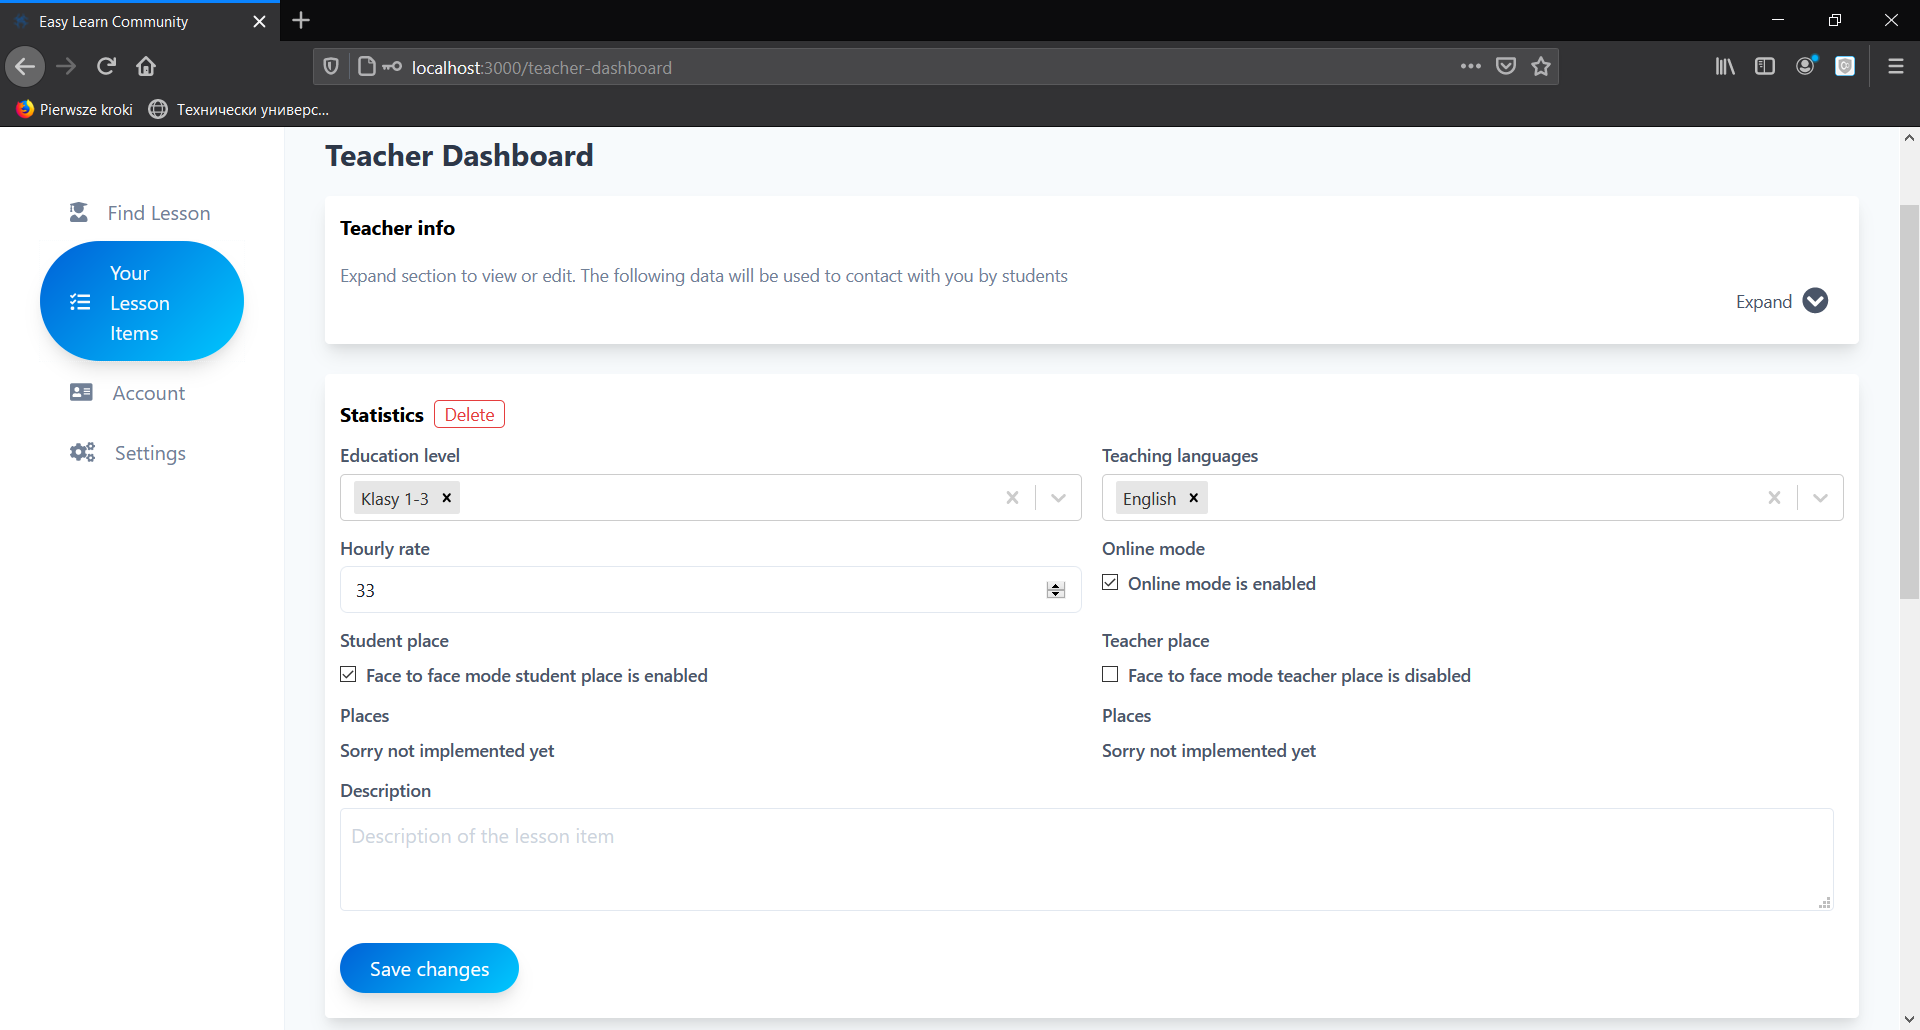
\includegraphics[width=\textwidth]{Include/Resources/Frontend/TeacherDashboard.png}
    \caption{Teacher dashboard} 
    \label{fig:TeacherDashboard}
\end{figure}

Admin account allows to manage all lesson items \textit{Lesson Items Administration} and users accounts \textit{Users}(figure nr \ref{fig:Admin})

\begin{figure}[H]
    \centering
    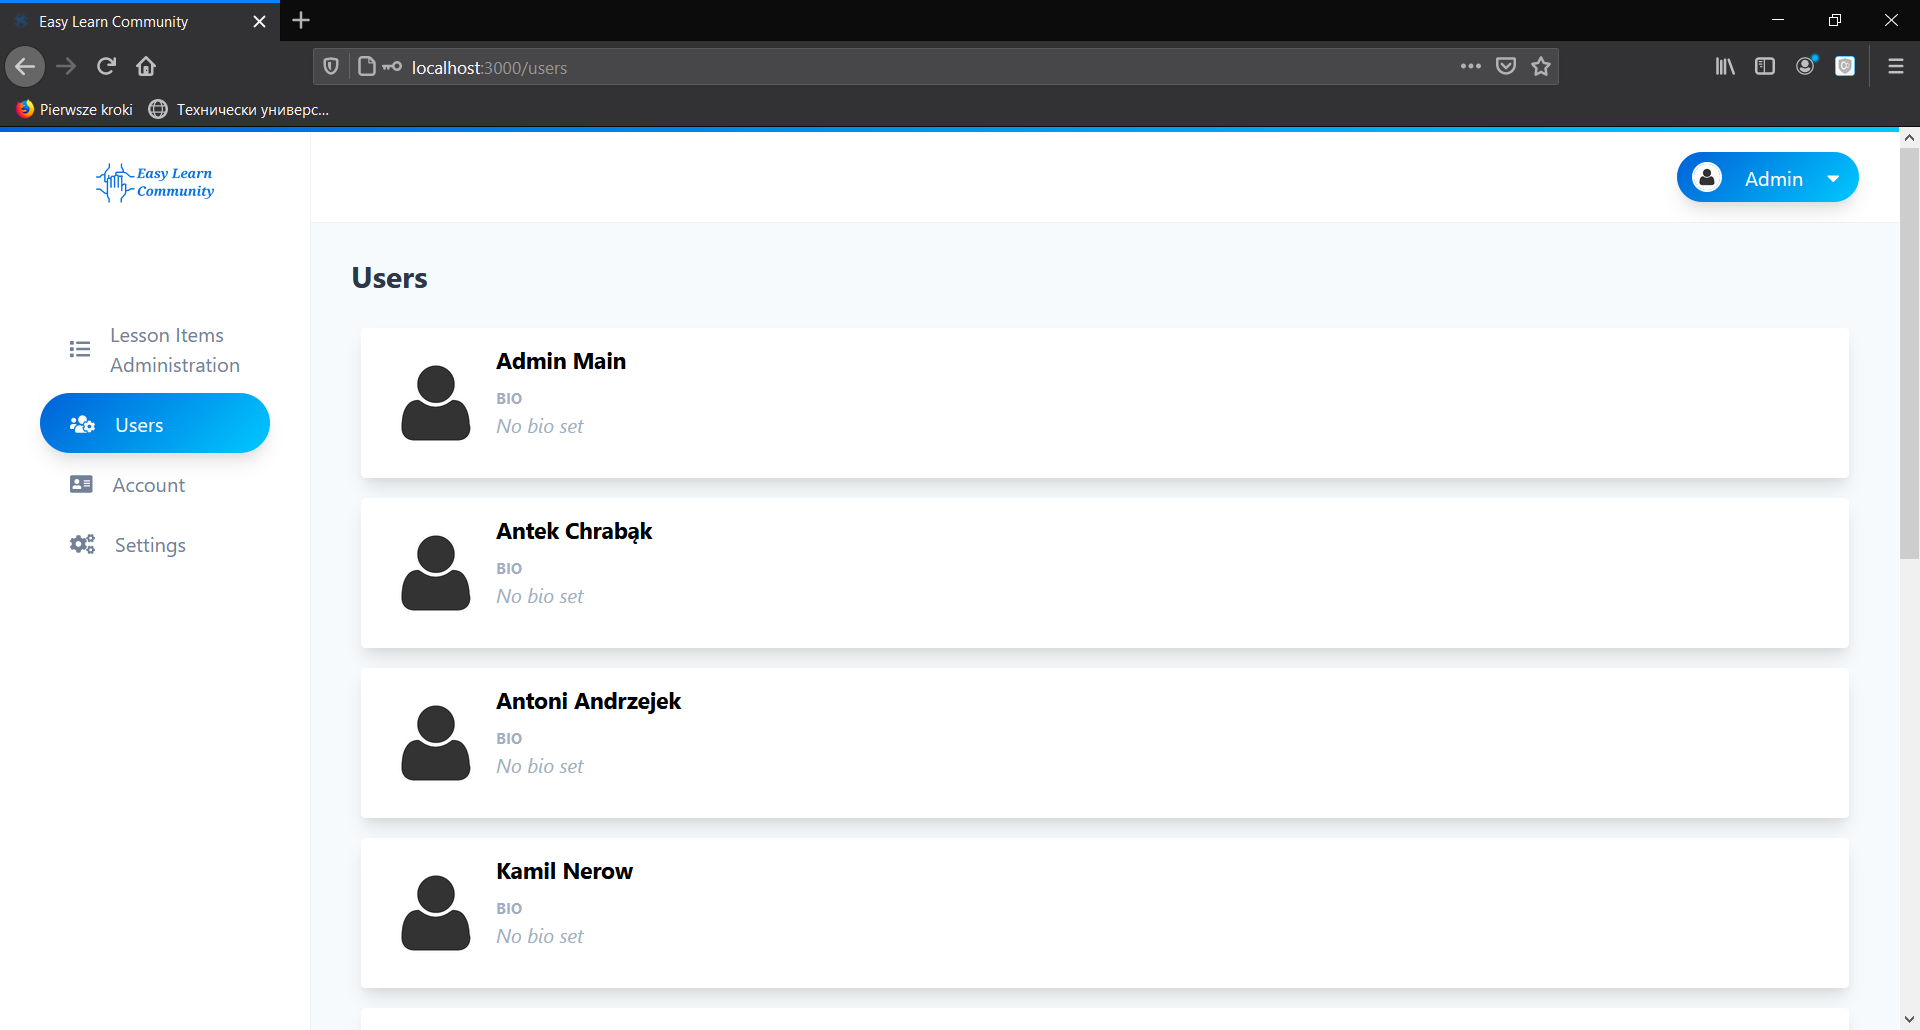
\includegraphics[width=\textwidth]{Include/Resources/Frontend/Admin.png}
    \caption{Become a teacher - add new lesson item} 
    \label{fig:Admin}
\end{figure}

Every user is allowed to change \textit{Personal Info}, \textit{Sensitive data} and set new password \textit{Change password}(figure nr \ref{fig:Account})

\begin{figure}[H]
    \centering
    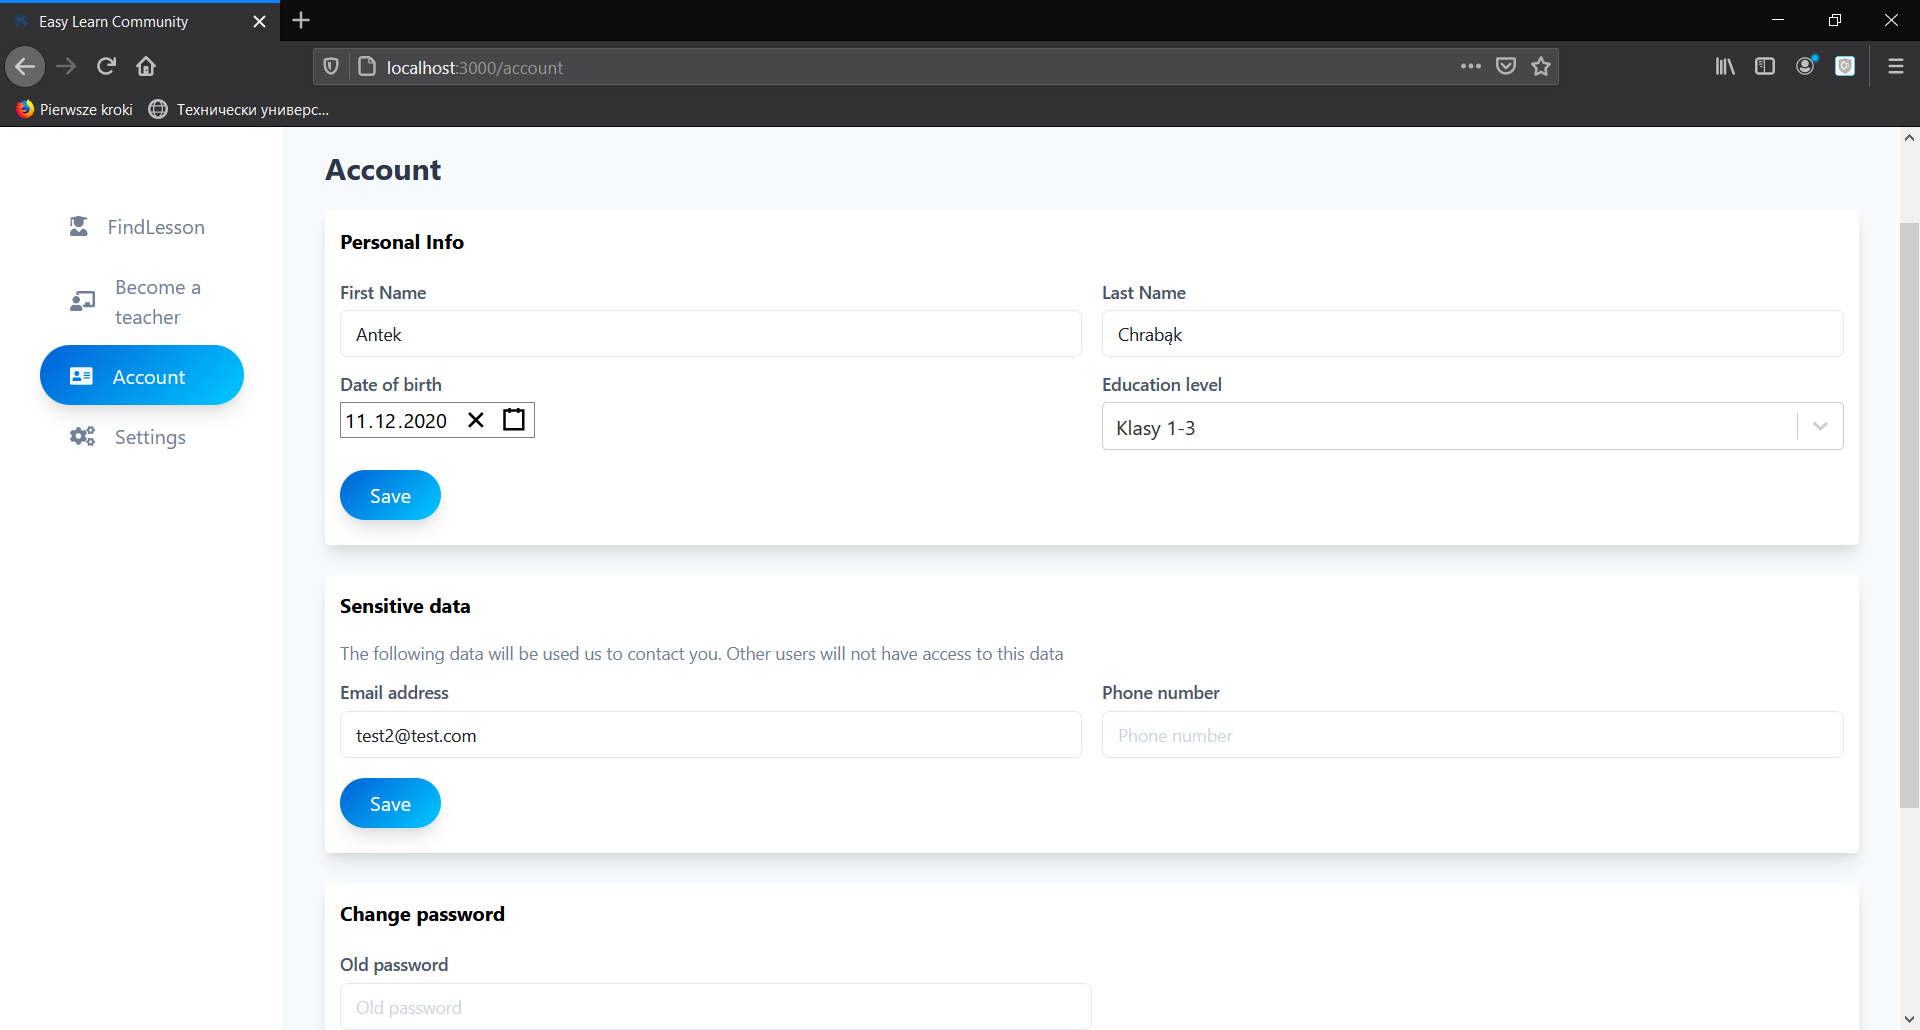
\includegraphics[width=\textwidth]{Include/Resources/Frontend/Account.png}
    \caption{Account settings} 
    \label{fig:Account}
\end{figure}

% \begin{figure}[H]
%     \centering
%     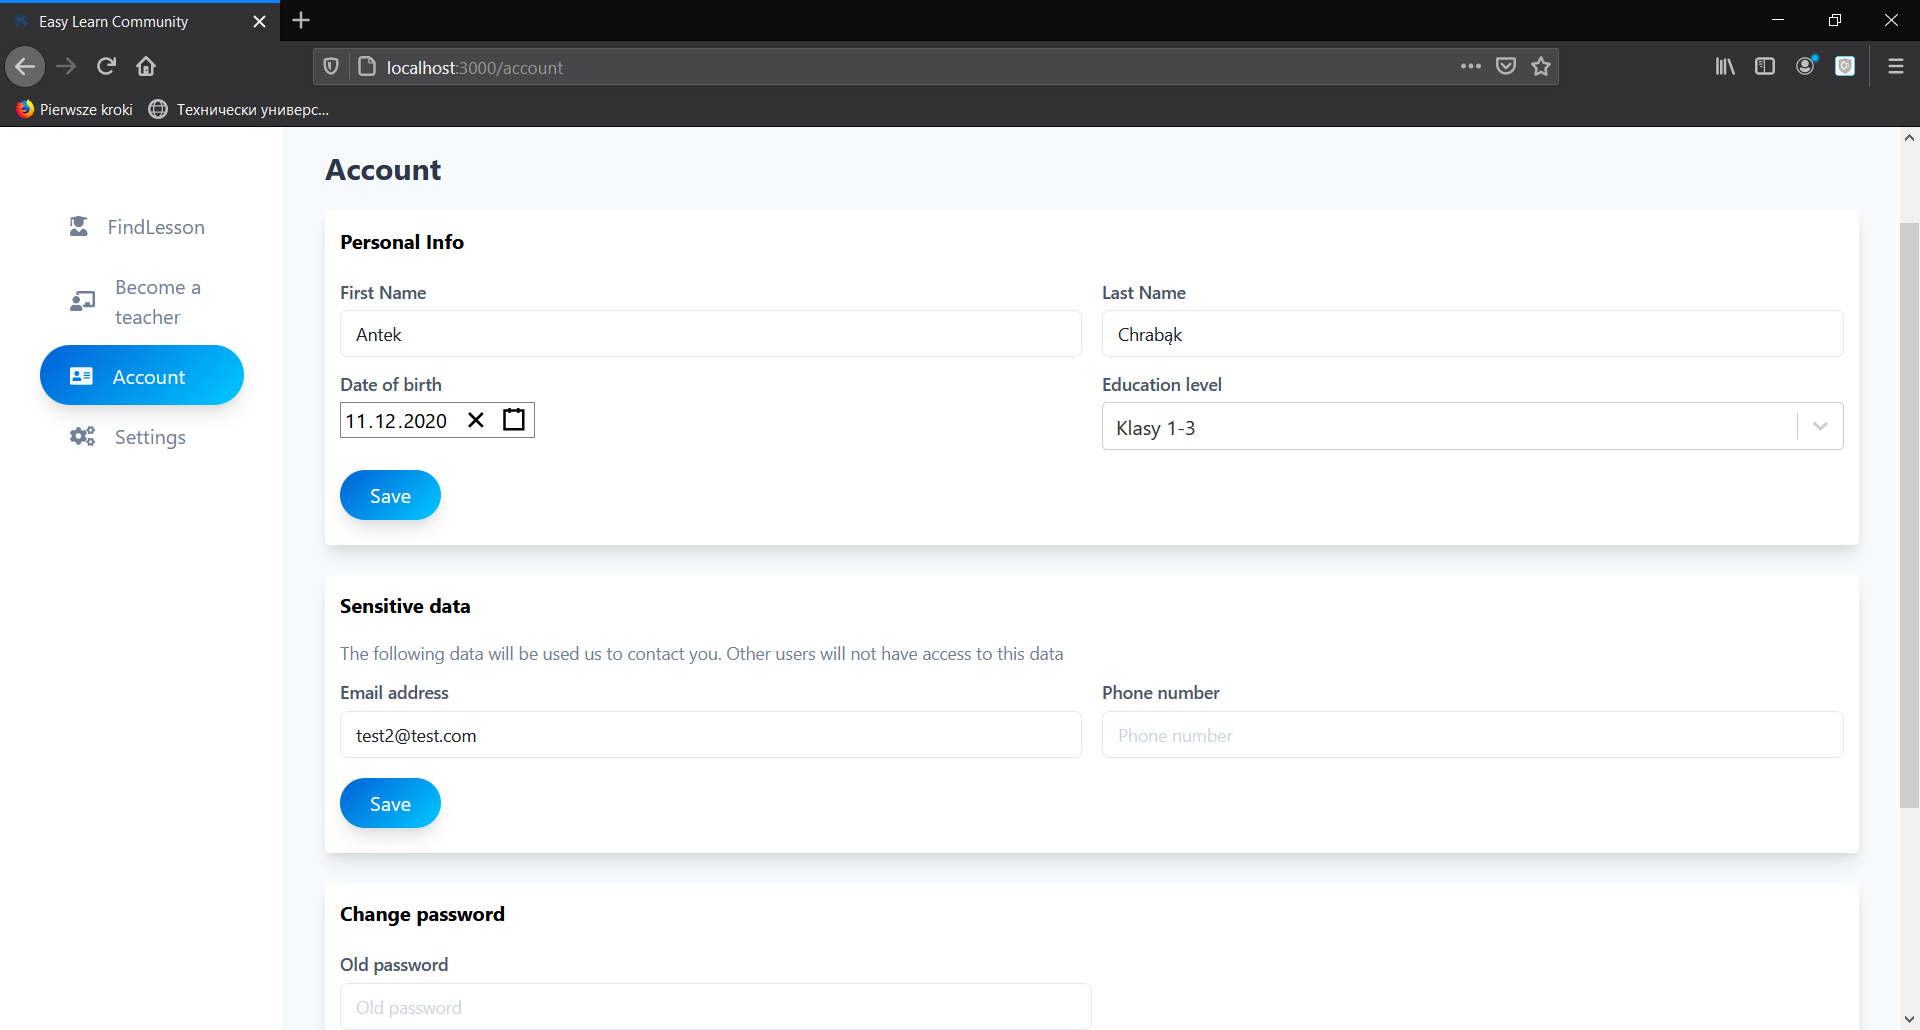
\includegraphics[width=\textwidth]{Include/Resources/Frontend/Account.png}
%     \caption{MongoDB Compass}
%     \label{fig:MongoDBCompass}
% \end{figure}

% \begin{lstlisting}[breaklines=true, numbers=left, stepnumber=1]
% \end{lstlisting}